\chapter{Requirements and Constraints}\label{ch:requirements}
In this chapter all the requirements and constraints for the project (up to system level only) are derived, stated and further analysed as described in \Cref{sec:reqanalysissetup}.
All the Systems Engineering information contained and applied  in this chapter is derived from~\cite{dsePMSESlides1}.

After all the project stakeholders were identified in \Cref{sec:Stakeholder_Analysis}, stakeholder needs were established and formulated into \enquote{shall} statements so that the Requirements Discovery Tree (RDT) of \Cref{fig:requirement-discovery-tree} could be constructed.
Once set up in the brainstorming phase of the requirements generation, the RDT proved as a useful tool to help identify all mission and system requirements; mission requirements \enquote{flow} from stakeholder requirements, and system requirements \enquote{flow} from mission requirements (STK<MIS<SYS structure).
The requirements are presented in the sections below, following from the structure of the RDT: requirements are split into technical (in \Cref{sec:technical-requirements}) and those stemming from mission constraints (\Cref{sec:constraints}).
The requirement identifiers are also given according to the \enquote{flow-down} structure of the RDT, given it is an \enquote{AND} tree.
For instance, the origin of requirement~\ref{Te-2-STK07-5-3} can be determined following its path from left to right in \Cref{fig:requirement-discovery-tree}, and following the IDs of the parent boxes as shown below in \Cref{fig:reqflow}:

\begin{figure}[H]
    \centering
    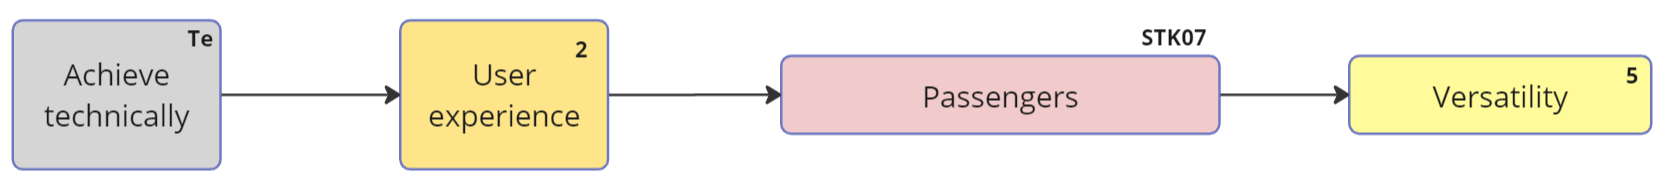
\includegraphics[width=\linewidth]{figures/reqflow.png}~\caption{Flow-down path of \textit{\ref{Te-2-STK07-5-3}}}
    \label{fig:reqflow}
\end{figure}

As the project is still in its early development and conceptual design phases, requirement generation stopped at the system level, hence not yet going into detailed subsystem requirements; moreover, some requirements contain TBD values as no precise figures could be exactly determined or computed at this stage.
\paragraph{Requirement origin}Information on requirement origin (stakeholder, mission or system requirement) can be easily derived by the ID length in \Cref{tab:technicalreq} and \Cref{tab:constrreqfinal}: one number after the stakeholder ID (stakeholder requirement level) indicates a mission requirement, whereas two numbers after the stakeholder ID indicate a system requirement.
This follows from the STK<MIS<SYS structure of the RDT as described at the beginning of the present chapter.

\paragraph{Requirement type}Division of the requirements in operational, functional and constraints will be explained in \Cref{sec:technical-requirements} and \Cref{sec:constraints}.

\section{Requirement Analysis}
\label{sec:reqanalysissetup}
After all the requirements were generated, they were manually inspected and analysed in order to determine which ones would be considered killer requirements, driving requirements and thus key requirements (either killer or driving).
Two killer requirements were identified at this stage of the conceptual design: \textit{Te-2-STK07-1-2} and \textit{Te-2-STK07-5-2}, both highlighted in red in \Cref{tab:technicalreq}.
Such requirements were deemed to be killer as the literature study showed how such figures are hard to achieve for similar aircraft (eVTOLs), therefore likely posing excessive engineering challenges on this project, greatly restricting the design space and requiring an unacceptably high portion of the available resources in order to be achieved.
Lower values following those found in literature will be defined and further proposed to the customers (who set these requirements) asking for renegotiation.

On the other hand, twenty-one key requirements were identified and highlighted in \textbf{green} within the tables.
Such requirements will need constant and careful monitoring over the course of the project.

Ultimately, the so-generated preliminary requirements were validated according to \enquote{VALID} (Verifiable, Achievable, Logical, Integral, Definite) criteria, resulting in a set of validated requirements to be used for the mission. 
It is important to note that not all top-level stakeholder requirements (third and fourth level in \Cref{fig:requirement-discovery-tree}) could be validated on their own, as some are not formulated in a SMART (Specific, Measurable, Achievable, Relevant, Time-bound) way, being too general.
Therefore, such requirements are said to be validated only when their children are individually validated.
Being the RDT an \enquote{AND} tree, every requirement is satisfied when its children are, backing the previous validation strategy.
Following such procedure, all the requirements in \Cref{tab:technicalreq} and \Cref{tab:constrreqfinal} were successfully validated.

\section{Technical Requirements}\label{sec:technical-requirements}
In \Cref{tab:technicalreq} the \textbf{technical} requirements (those originating from the \enquote{Achieve technically} box, with ID \textit{Te} in \Cref{fig:requirement-discovery-tree}) will be presented. \textbf{Technical} (or \textbf{functional}) requirements define what a system is supposed to do and how well it must do it, therefore directly limiting the workspace of the project from a functional \enquote{what is needed to be achieved technically to perform the mission}-point of view.
A subset of the \textit{Te} branch is the \textbf{operational} requirements, stemming from block \textit{Te-1}, defining how the system is to be used by the stakeholders with a direct interest in operating/handling the vehicle (namely \textit{STKO3}, \textit{STK06}, \textit{STK04} in \Cref{tab:stakeholders}).
% \begin{table}[H]
%     \centering
%     \caption{Technical requirements}
%     \label{tab:technicalreq}
    \begin{longtable}{m{0.16\linewidth}m{0.74\linewidth}}
    \caption{Technical requirements}
    \label{tab:technicalreq}
        \\\hline &~\textbf{Air taxi operators (\ref{stk:ato})} \\\hline
        Te-1-\ref{STK03} & The vehicle shall comply with the operational wishes of air taxi operators. \\
            Te-1-\ref{STK03}-1 & The vehicle shall be fully charged within TBD[min].\\
                \cellcolor[HTML]{9AFF99}Te-1-\ref{STK03}-1-1& \cellcolor[HTML]{9AFF99}The vehicle shall be able to charge at a minimum power of TBD[W].\\
            Te-1-\ref{STK03}-2 & The vehicle shall not require scheduled maintenance procedures more often than every TBD months. \\
            
            
%             \end{longtable}
% \end{table}

% \begin{table}[H]
%     \centering
%     \begin{longtable}{m{0.16\linewidth}m{0.74\linewidth}}  
        \cellcolor[HTML]{9AFF99}Te-1-\ref{STK03}-3 & \cellcolor[HTML]{9AFF99}The vehicle shall be able to carry at least 400[kg] of payload.\\
        Te-1-\ref{STK03}-4 & The pilot training efforts for the mission shall be minimised or eliminated \\
            \cellcolor[HTML]{9AFF99}Te-1-\ref{STK03}-4-1 & \cellcolor[HTML]{9AFF99}The vehicle shall be able to fly autonomously. \\
        \hline &~\textbf{Maintenance contractors (\ref{stk:maintenance-contractors})} \\\hline
        Te-1-\ref{STK06} & The vehicle shall comply with the operational wishes of maintenance contractors. \\
        Te-1-\ref{STK06}-1 & Correct engineering drawings, which follow the internationally accepted conventions, shall be produced for each part, sub-assembly and assembly.\\
        Te-1-\ref{STK06}-2 & A complete and clear maintenance manual shall be provided. \\
        Te-1-\ref{STK06}-3 & The vehicle shall be easily maintainable.\\
        \cellcolor[HTML]{9AFF99}Te-1-\ref{STK06}-3-1 & \cellcolor[HTML]{9AFF99}The vehicle components requiring regular maintenance shall be easily accessible.\\
        Te-1-\ref{STK06}-3-2 & Each vehicle component shall be replaceable.\\
        \hline &~\textbf{Ground operators (\ref{stk:gso})} \\\hline
        Te-1-\ref{STK04} & The vehicle shall comply with the operational wishes of ground operators. \\
        Te-1-\ref{STK04}-1 & The cargo department shall be easily accessible from the ground.\\
        Te-1-\ref{STK04}-2 & Ground operations shall be performable by TBD people within TBD[min]. \\
        Te-1-\ref{STK04}-3 & The vehicle shall be equipped with robust safety features that protect ground staff and equipment.\\
        Te-1-\ref{STK04}-3-1 & The vehicle shall preserve the integrity of the vertiport upon take-off and landing.\\
        Te-1-\ref{STK04}-3-2 & The vehicle shall be equipped with an emergency engine-propeller decoupling system, when non-operational.\\
%     \end{longtable}
% \end{table}
% \begin{table}[H]
%     \centering
%     \begin{longtable}{m{0.18\linewidth}m{0.72\linewidth}}
        \hline &~\textbf{Passengers (\ref{stk:passengers})} \\\hline
        Te-2-\ref{STK07} & The vehicle shall provide a satisfactory user experience for its passengers. \\
        Te-2-\ref{STK07}-1 & The vehicle shall be comfortable for passengers. \\
        Te-2-\ref{STK07}-1-1 & The cabin seats shall be adjustable. \\
        \cellcolor[HTML]{FD6864}Te-2-\ref{STK07}-1-2 & \cellcolor[HTML]{FD6864}The noise level within the cabin shall never exceed 60 [dBA].\\
        Te-2-\ref{STK07}-1-3 & The leg space between one seat and the other shall be at least TBD[\unit{m}].\\
        \cellcolor[HTML]{9AFF99}Te-2-\ref{STK07}-1-4 & \cellcolor[HTML]{9AFF99}The load factor experienced during flight shall be kept at all times within 0.7 [g] and 1.3 [g] \footnote{[g]=\qty{9.80665}{\m\per\s^2}}.\\
        Te-2-\ref{STK07}-1-5 & The inside cabin height shall be of at least TBD[\unit{\m}].\\
        \cellcolor[HTML]{9AFF99}Te-2-\ref{STK07}-2 & \cellcolor[HTML]{9AFF99}The vehicle cabin shall be easily accessible for passengers. \\
        Te-2-\ref{STK07}-2-1 & The cabin door dimensions shall be at least of TBD x TBD [\unit{\m}]. \\
        Te-2-\ref{STK07}-2-2 & The cabin also shall be accessible by passengers with disabilities.\\
        Te-2-\ref{STK07}-3 & The vehicle shall allow for low travel times. \\
        \cellcolor[HTML]{9AFF99}Te-2-\ref{STK07}-3-1 & \cellcolor[HTML]{9AFF99}The vehicle shall have a minimum flight block speed of TBD [\unit{\km\per\hour}].\\
        \cellcolor[HTML]{9AFF99}\newref{Te-2-\ref{STK07}-3-2}\label{Te-2-STK07-3-2} & \cellcolor[HTML]{9AFF99}The vehicle shall have a cruise speed of 200 [\unit{\km\per\hour}]. \\

        Te-2-\ref{STK07}-4 & Vertiports shall be widely available.  \\
        Te-2-\ref{STK07}-4-1 & In areas of implementation, vertiports shall be located a maximum TBD[\unit{\km}] apart. \\
        Te-2-\ref{STK07}-5 & The vehicle shall be able to fly at least 345 days a year. \\
        Te-2-\ref{STK07}-5-1 & The vehicle shall be able to fly at night.\\
        
        \cellcolor[HTML]{FD6864}Te-2-\ref{STK07}-5-2 & \cellcolor[HTML]{FD6864}The vehicle shall be able to withstand winds of up to 8 Beaufort.\\
        \cellcolor[HTML]{9AFF99}\newref{Te-2-\ref{STK07}-5-3}\label{Te-2-STK07-5-3} & \cellcolor[HTML]{9AFF99}The vehicle shall be capable of flying in rainy conditions.\\ \hline
    \end{longtable}
%\end{table}

\section{Constraints}
\label{sec:constraints}
In this section \Cref{tab:constrreqfinal}, containing the requirements originating from constraints set by the various stakeholders (namely those originating from the \enquote{Achieve within constraints} box, with ID \textit{Co} in \Cref{fig:requirement-discovery-tree}), will be presented.
% \begin{table}[H]
%     \centering
%     \caption{Requirements deriving from constraints}
%     \label{tab:constraintsreq}
    \begin{longtable}{m{0.17\linewidth}m{0.74\linewidth}}
    \caption{Constraint requirements}
    \label{tab:constrreqfinal}
        \\\hline &~\textbf{Private costumers (\ref{stk:private-costumers})} \\ \hline
        Co-1-\ref{STK05} & The vehicle shall be economically viable for private customers . \\
        \cellcolor[HTML]{9AFF99}Co-1-\ref{STK05}-1 & \cellcolor[HTML]{9AFF99}The vehicle cost of production per unit shall be less than 2000k[€]. \\

        \hline &~\textbf{Airtaxi operators (\ref{stk:ato})} \\\hline
         Co-1-\ref{STK03} & The vehicle shall be economically viable for airtaxi operators. \\
                        Co-1-\ref{STK03}-1 & The operational costs shall be minimised. \\
            Co-1-\ref{STK03}-2 & The vehicle public market price for airtaxi operators shall be less than TBD[€]. \\

        \hline &~\textbf{Passengers (\ref{stk:passengers})} \\\hline
        Co-1-\ref{STK07} & The vehicle shall allow economically viable travelling costs. \\
        Co-1-\ref{STK07}-1 & Fair prices of vehicle services shall not exceed TBD[€/km]. \\
       \hline  &~\textbf{Investors (\ref{stk:investors})} \\\hline
        Co-2-\ref{STK01} & The investors' needs shall be satisfied throughout the project.\\
            Co-2-\ref{STK01}-1 & The investors shall be provided with a return on investment plan.\\
            Co-2-\ref{STK01}-2 & The investors shall be informed about the progress at each phase of the project.\\
            Co-2-\ref{STK01}-3 & The investors shall be provided with risk reports.\\
            Co-2-\ref{STK01}-4 & The investor shall be provided with clear documentation regarding budget allocation. \\
        \hline &~\textbf{Delft University of Technology (TU Delft) (\ref{stk:tud})} \\ \hline
        Co-2-\ref{STK02} & The TU Delft and its associated parties shall be fully respected.\\
            Co-2-\ref{STK02}-1 & The contributors to the project from TU Delft shall be acknowledged.\\
            Co-2-\ref{STK02}-2 & The project must be carried out under TU Delft regulations.\\
            Co-2-\ref{STK02}-3 & The project must be carried out respecting TU Delft values.\\
            Co-2-\ref{STK02}-4 & Vehicle shall be designed in 10 weeks time.\\
        \hline &~\textbf{Passengers (\ref{stk:passengers})} \\\hline
        Co-3-\ref{STK07} & The safety needs of passengers shall be taken into account. \\
        \cellcolor[HTML]{9AFF99}Co-3-\ref{STK07}-1 & \cellcolor[HTML]{9AFF99}The vehicle predicted reliability shall be of maximum one failure per million flight hours ($\text{10}^{-6}$ reliability)~\cite{106safety}. \\

        \hline &~\textbf{Air-taxi operators (\ref{stk:ato})} \\\hline
         Co-3-\ref{STK03} & The vehicle shall comply with the wishes of Air-taxi operators regarding safety. \\
      
        \cellcolor[HTML]{9AFF99}\newref{Co-3-\ref{STK03}-1}\label{Co-3-STK03-1} & \cellcolor[HTML]{9AFF99}The vehicle shall be able to fly with only 75\% of the propulsion system working. \\



        \hline &~\textbf{Environmental organisations (\ref{stk:environmental-orgs})} \\\hline
         Co-4-\ref{STK13} & The vehicle shall not interfere with the agendas of environmental organisations over its full lifecycle.\\
         Co-4-\ref{STK13}-1 & Operating the vehicle shall have a low environmental and ground footprint.\\
         \cellcolor[HTML]{9AFF99}Co-4-\ref{STK13}-1-1 & \cellcolor[HTML]{9AFF99}The vehicle shall be fully electric. \\
        Co-4-\ref{STK13}-1-2 & The manufacturing processes shall reduce waste production by TBD\% compared to TBD. \\
        Co-4-\ref{STK13}-1-3 & The building materials shall be sourced from recycled or sustainable sources for at least TBD\%. \\
        \cellcolor[HTML]{9AFF99}\newref{Co-4-\ref{STK13}-1-4}\label{Co-4-STK13-1-4} & \cellcolor[HTML]{9AFF99}The vehicle shall have maximum dimensions of 8x4x2 $[m^3]$ on the ground. \\
        \cellcolor[HTML]{9AFF99}Co-4-\ref{STK13}-1-5 & \cellcolor[HTML]{9AFF99}The vehicle shall have a lifetime greater than 10 years. \\
        \cellcolor[HTML]{9AFF99}Co-4-\ref{STK13}-1-6	& \cellcolor[HTML]{9AFF99}The vehicle structure shall be reusable for at least 10 years after its life. \\
         Co-4-\ref{STK13}-2 & The vehicle shall not result in non-recyclable waste at its end-of-life.\\
        Co-4-\ref{STK13}-2-1 & The vehicle components shall be easily recyclable. \\
        Co-4-\ref{STK13}-2-2 & The vehicle shall be easy to dismantle. \\
        Co-4-\ref{STK13}-2-3 & All the vehicle batteries shall be reused and/or regenerated at the end-of-life of the vehicle. \\

        \hline &~\textbf{EU government (\ref{stk:EU})} \\\hline
         Co-4-\ref{STK15} & The vehicle shall contribute to achieving the goals for sustainable commercial aviation set by the EU. \\
%          \end{longtable}
% \end{table}

% \begin{table}[H]
%     \centering
%     \begin{longtable}{m{0.16\linewidth}m{0.74\linewidth}}
         Co-4-\ref{STK15}-1 & Energy consumption of the operating vehicle shall be reduced to the optimal minimum. \\
        Co-4-\ref{STK15}-1-1 & The vehicle shall follow an optimal flight route. \\
        
        Co-4-\ref{STK15}-2 & The vehicle shall operate in full compliance with EU environmental standards, regulations, and proposals. \\
        Co-4-\ref{STK15}-2-1 & Systems for real-time monitoring and reporting of emissions that comply with EU standards shall be implemented in the system.\\
        Co-4-\ref{STK15}-2-2 &	A life cycle assessment shall be performed.\\
    
        \hline &~\textbf{Affected public (\ref{stk:affected-public})} \\\hline
        Co-5-\ref{STK14}&  The project shall attempt to gain the affected public's acceptance.\\
        Co-5-\ref{STK14}-1	& The vehicle shall not disturb citizens. \\
        \cellcolor[HTML]{9AFF99}Co-5-\ref{STK14}-1-1& 	\cellcolor[HTML]{9AFF99}The noise level at TBD[m] from the vehicle shall not exceed TBD[dB]. \\
        Co-5-\ref{STK14}-1-2 &	The vehicle shall fly over highways and water as much as possible. \\
        Co-5-\ref{STK14}-2 & The vehicle not be hazardous to the citizens. \\
        Co-5-\ref{STK14}-2-1 &	The vehicle shall be able to safely operate at 5[m] distance from people. \\
        Co-5-\ref{STK14}-2-2 & The vehicle shall keep a safety distance of at least 3[m] from any object in populated areas. \\

        \hline &~\textbf{General public (\ref{stk:general-public})} \\\hline
        Co-5-\ref{STK18}& The project shall attempt to gain the general public's acceptance. \\
        Co-5-\ref{STK18}-1	& The vehicle shall not contribute to the \enquote{horizon vervuiling}. \\
        \hline &~\textbf{National government (\ref{stk:national-govs})} \\ \hline
        Co-5-\ref{STK16} & The vehicle shall not compromise the country's reputability.  \\
        Co-5-\ref{STK16}-1 & The vehicle shall facilitate transport between cities. \\
        \cellcolor[HTML]{9AFF99}\newref{Co-5-\ref{STK16}-1-1}\label{Co-5-STK16-1-1} & \cellcolor[HTML]{9AFF99}The vehicle shall have an electric power autonomy of \qty{100}{km} plus reserve.\\

        \hline &~\textbf{Airfields (\ref{stk:airfield})} \\\hline
        Co-6-\ref{STK20} & The vehicle shall conform with airfield regulations.\\
        Co-6-\ref{STK20}-1 & The vehicle shall not disturb current airfield operations.\\
        Co-6-\ref{STK20}-1-1 & The vehicle shall not fly within a range of TBD[km] from airfields.\\
        \hline &~\textbf{Energy providers (\ref{stk:energy-providers})} \\\hline
        Co-6-\ref{STK19} & The vehicle and its operations shall comply with the needs and standards of energy providers.\\
        Co-6-\ref{STK19}-1 & The charging framework shall comply with standards readily used in the industry.\\
        Co-6-\ref{STK19}-1-1 & The charging system shall be capable of updating or upgrading following changes in industry standards every TBD[years].\\
        Co-6-\ref{STK19}-1-2 & Off-the-shelf charging components shall be used whenever possible.\\
        Co-6-\ref{STK19}-2 & The vertiports shall not burden the electricity network. \\
        Co-6-\ref{STK19}-2-1 & Privately owned vehicles shall be only charged overnight.\\
        Co-6-\ref{STK19}-2-2 & Vertiports with charging capabilities shall be placed taking grid capacities into account.\\
        \hline &~\textbf{Air traffic control (\ref{stk:atc})} \\\hline
        Co-6-\ref{STK12} & The vehicle shall conform to air traffic control regulations, protocols, and standards.\\
        Co-6-\ref{STK12}-1 & The vehicle shall adhere to the requirements and standards set by EUROCONTROL.\\
        Co-6-\ref{STK12}-1-1 & The automatic communications system of the vehicle shall follow the protocols specified by EUROCONTROL.\\
        Co-6-\ref{STK12}-2 & The vehicle shall be capable of all necessary communication capabilities.\\
        Co-6-\ref{STK12}-2-1 & The vehicle shall be equipped with the necessary communication instruments.\\
        \hline &~\textbf{Municipalities (\ref{stk:municipalities})} \\\hline
        Co-6-\ref{STK17} & The vehicle and its operations shall comply with the wishes and regulations of EU municipalities.\\
%         \end{longtable}
% \end{table}

% \begin{table}[H]
%     \centering
%     \begin{longtable}{m{0.17\linewidth}m{0.74\linewidth}}        
        Co-6-\ref{STK17}-1 & Vertiports shall have a low ground footprint.\\
        Co-6-\ref{STK17}-1-1 & The vertiport dimensions shall not exceed TBD x TBD [m].\\
        Co-6-\ref{STK17}-2 & Vertiports shall not compromise the attractiveness of the municipality.\\
        \hline &~\textbf{EU government (\ref{stk:EU})} \\\hline
        Co-6-\ref{STK15} & The vehicle shall adhere to the regulations of the EU.\\
        Co-6-\ref{STK15}-1 & The vehicle shall adhere to the EU Taxonomy Regulation~\cite{eu-taxonomy}.\\ \hline
    \end{longtable}
%\end{table}

\afterpage{
    \clearpage
    \thispagestyle{empty}
    \KOMAoptions{paper=A3,paper=landscape,pagesize}
    \recalctypearea

    \begin{figure}
        \centering
        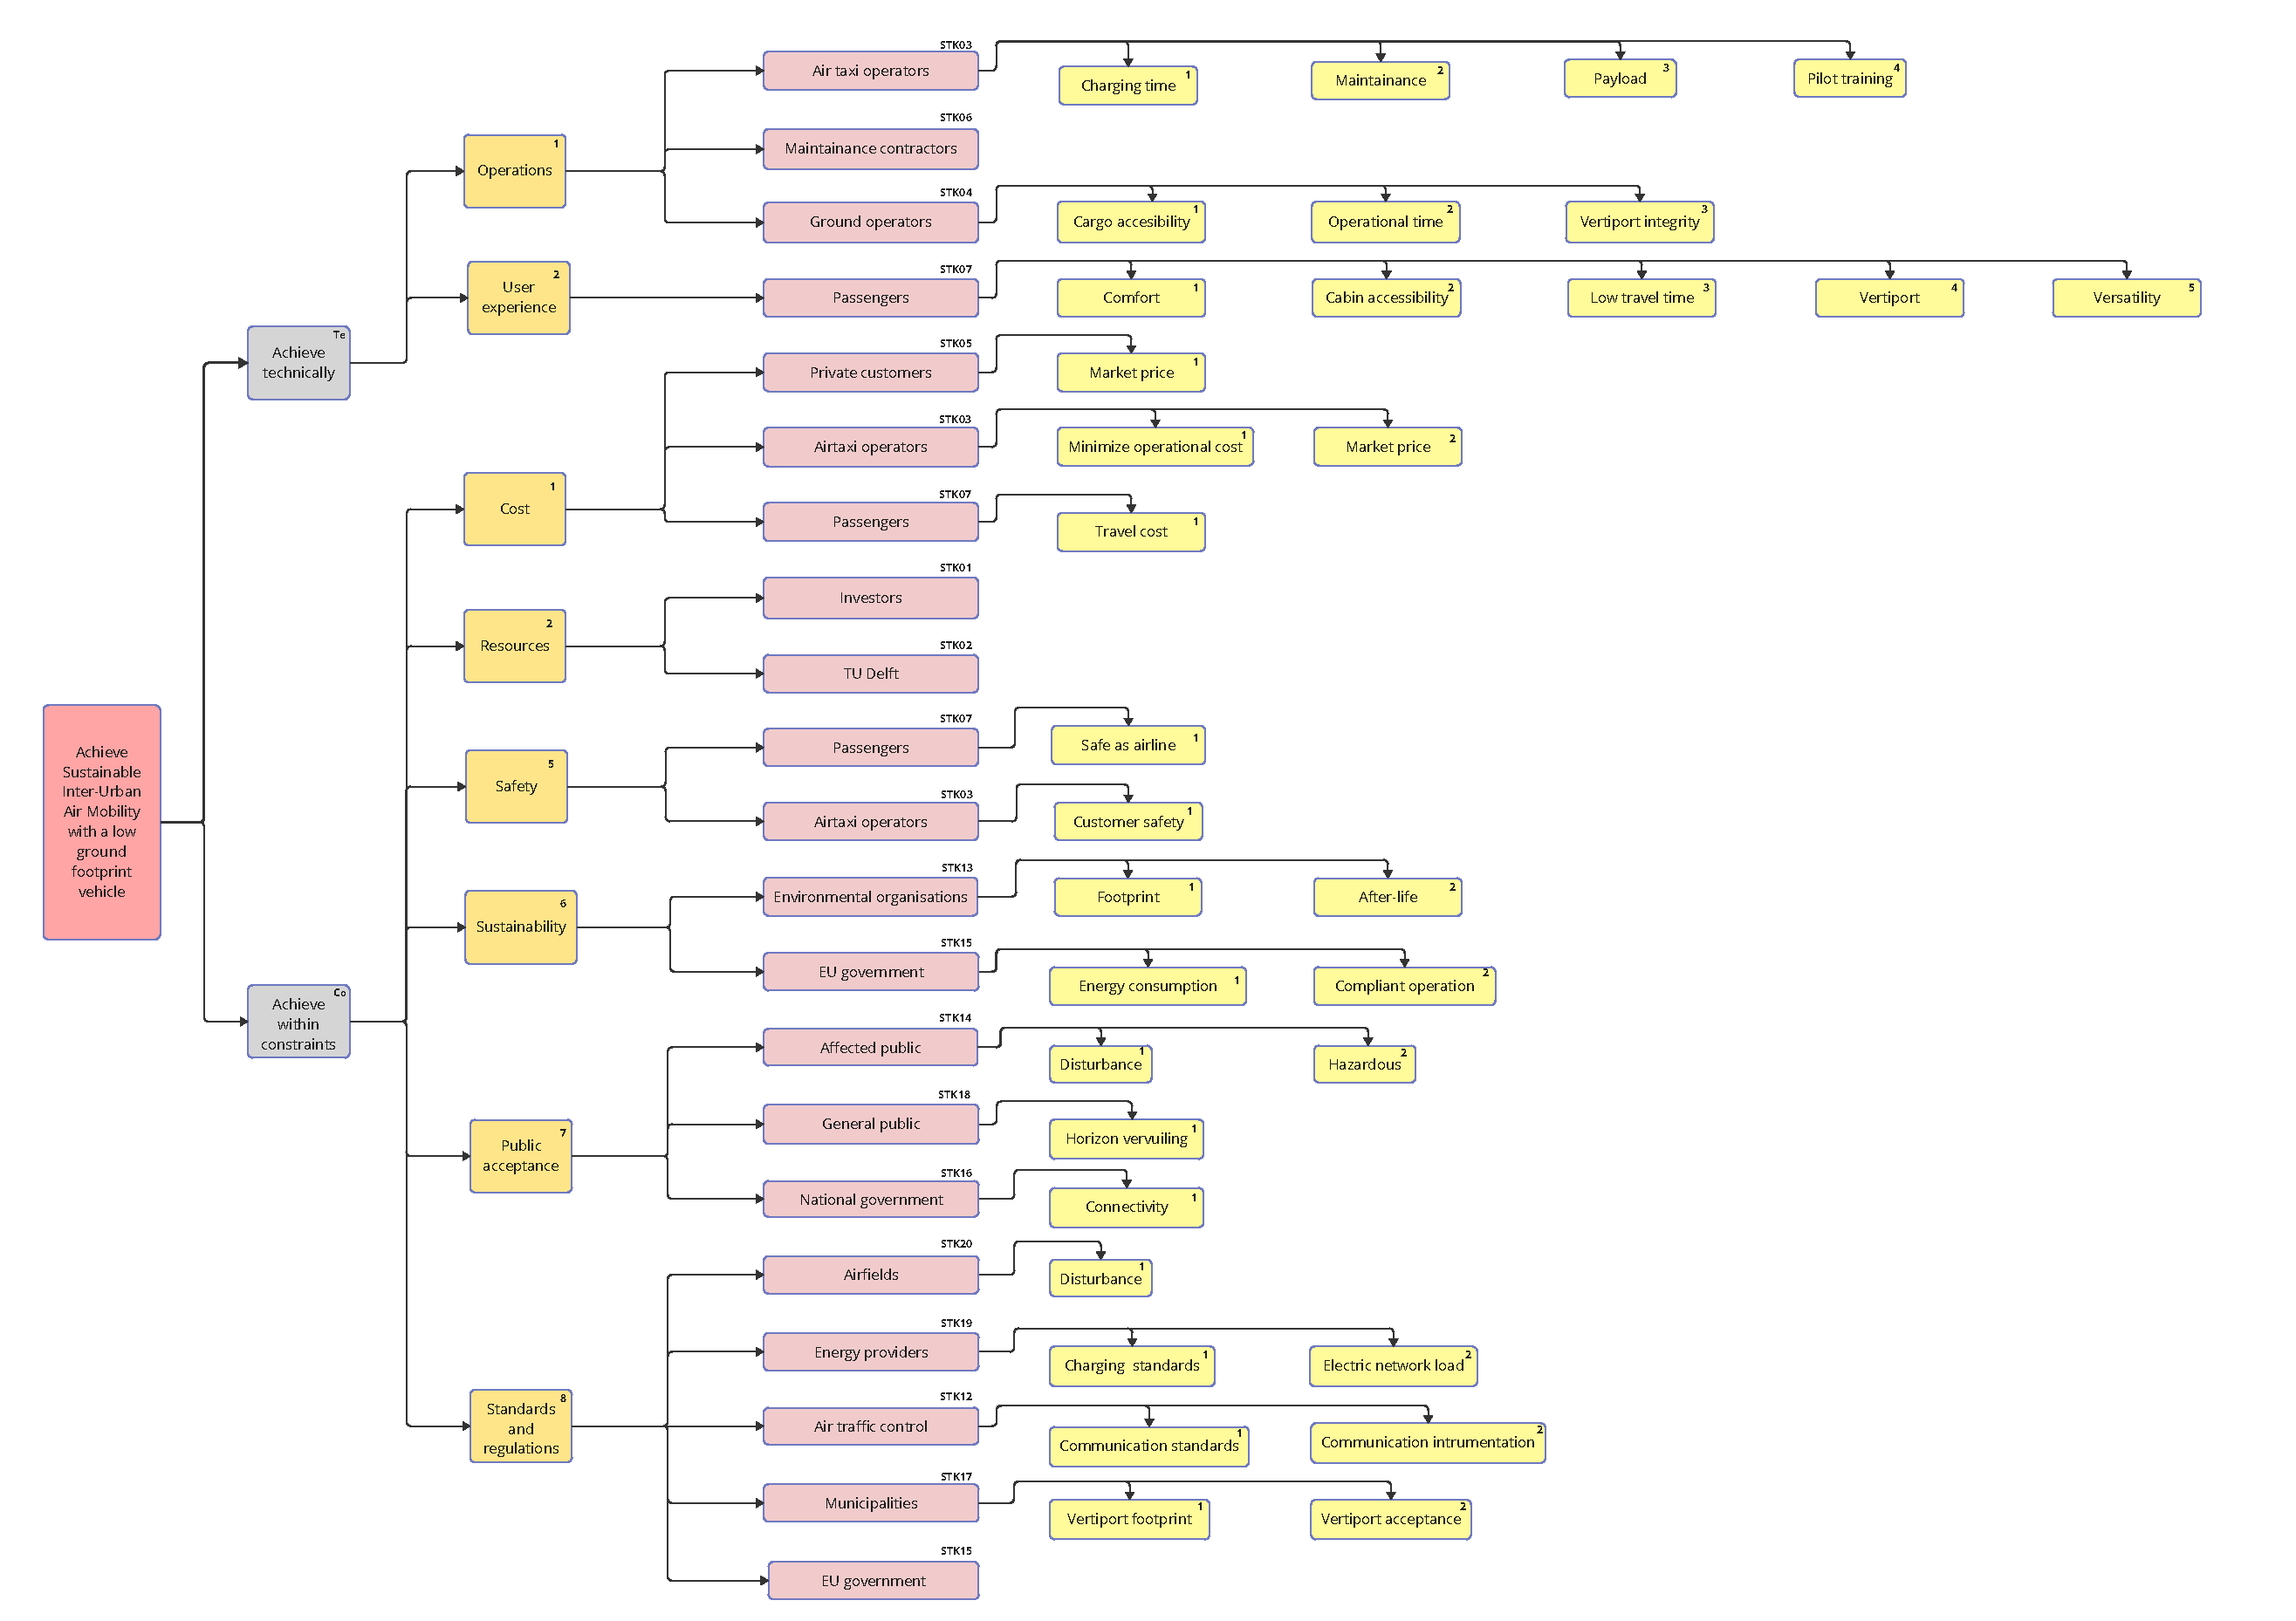
\includegraphics[width=1.1\linewidth]{figures/Requirements/requirement_discovery_tree_v1.pdf}
        \caption{Requirement Discovery Tree}
        \label{fig:requirement-discovery-tree}
    \end{figure}

    \clearpage
    \KOMAoptions{paper=A4,paper=portrait,pagesize}
    \recalctypearea
}



